% vim: spell spelllang=en_gb
\chapter{Literature Review}

The massive and accessible volume of data produced by social media has attracted the attention of
many researchers as a valuable data source for their research topic; however, collecting and
processing data of this nature pose many challenges to extracting useful information. This section
mentions what other researchers focusing on disaster management topics did to address these
challenges while using Twitter; it also discusses the different approaches used for identifying
relevant tweets, extracting geographical location from them, making text analysis on the text, and visualizing the results.

\section{Data Collection} 

Twitter's \ac{API} enables developers to retrieve historical tweets using queries that are made of
operators to match a variety of tweet attributes, such as a specific keyword, having a geotag
provided by the user who created the tweet, and the language classified by Twitter. Users generate
around 500-700 million tweets a day \cite{inproceedings}, making it necessary to limit the number of
tweets to fetch using the \ac{API} to reduce computational power and downtime.
\citeauth{fengExtractionPluvialFlood2018} fetch geotagged tweets and filter them using 45 keywords
in 7 languages; this approach disregards a massive portion of relevant tweets since 1\% of tweets
are geotagged \cite{middletonRealTimeCrisisMapping2014}. A better way that doesn't only regard 1\%
of the tweets is to fetch tweets using keywords related to the topic of interest in different
languages. \citeauth{debruijnGlobalDatabaseHistoric2019b} use over 40 keywords associated with
floods in 11 major languages in the query to fetch tweets.

In addition to textual data, some researchers use other data types to enhance their pipelines. Some
tweets contain media attachments, such as images and videos that potentially provide additional
visual information for the concerned research topic
\cite{alamFloodDetectionTwitter2020}\cite{ningPrototypingSocialMedia2020}\cite{saidFloodsDetectionTwitter2020};
search engines are another resourceful source for images as well
\cite{fengExtractionPluvialFlood2018}. For flooding events, hydrological information can be a
valuable source of information, which can be extracted from a global precipitation dataset based on
tweets' time stamps and location in the text \cite{debruijnImprovingClassificationFlood2020}.
\citeauth{barkerDevelopmentNationalscaleRealtime2019} use Environment Agency flood-monitoring
\ac{API}\footnote{https://environment.data.gov.uk/flood-monitoring/doc/reference\#flood-warnings} to
get river gauge levels and flood warnings to identify at-risk flooding areas.

Text processing is crucial for any \ac{NLP} pipeline to train performant classifiers. Some research
deals with multilingual corpus, making it necessary to translate the text to one language (most
likely English) if the used classifier can not handle multilingual data
\cite{singhEventClassificationLocation2019}. One of the most common text-processing tasks is
removing unnecessary terms such as stopwords, \ac{URL}s, numbers, and punctuation marks. ``User
mentions'' (e.g. @user123) in tweets don't provide helpful information, so pipelines often remove or
replace them with a generic term, such as ``@user'' \cite{debruijnImprovingClassificationFlood2020}.
The location of the flood event is a crucial piece of information that can be pinpointed from a term
in the tweet, making it a potential target that includes bias in the dataset by overusing it;
\citeauth{debruijnImprovingClassificationFlood2020} replace these terms by the country name that
the location resides in; on the other hand, \citeauth{petersenIdentificationExplorationExtreme2021}
replace the terms by the word ``place'' if they get mentioned more than 0.5\% of the size of the
data set. Another way to improve the performance of the classifier is to group the terms by
converting them to lower-case and transforming them to their lexeme (e.g. better turns to good) or
word stem (e.g. walking turns to walk) by lemmatisation
\cite{petersenIdentificationExplorationExtreme2021} or stemming
\cite{fengExtractionPluvialFlood2018}, respectively.

 Some tweets are redundant or do not provide relevant information; these can be considered noise and
 filtered out. For example, retweets are identical to other tweets without additional context making
 them unneeded. Spam bots generate similar tweets for malicious reasons, such as spreading false
 content to manipulate the public, and utility reasons, such as creating a feed for users to check
 updates. These tweets introduce noise to the dataset that gets reduced by removing duplicate
 tweets. \citeauth{debruijnGlobalDatabaseHistoric2019b} only consider one tweet from each user in
 the last 14 days mentioning a specific region; they also discard tweets containing more than five
 consecutive words that match with those in another tweet among the previous 100 talking about a
 location. \citeauth{singhEventClassificationLocation2019} approach this problem by only extracting
 tweets created from mobile phones and only consider tweets from users who have $\text{followers} /
 \text{following} < 1$.

\section{Text Classification}
Identifying disaster events using social media requires a classifier to determine the relevant data.
Textual data containing terms related to a disaster doesn't mean it discusses a disastrous event
since words such as ``flood'' can be used figuratively in sentences (e.g., a flood of joy). A binary
classifier labelling the data with ``on-topic'' and ``off-topic'' labels is needed to filter out
irrelevant content.

Most classifiers use supervised \ac{ML} algorithms requiring labelled data for training. A
straightforward approach is to manually label a sample of the tweets
\cite{barkerDevelopmentNationalscaleRealtime2019}\cite{debruijnGlobalDatabaseHistoric2019b}.
\citeauth{petersenIdentificationExplorationExtreme2021} use CrisisLex6
\cite{olteanuCrisisLexLexiconCollecting2014}, a crowdsourced collection of labelled tweets, for
training their classifiers that get evaluated on 88 million unlabelled tweets containing
flood-related terms \cite{DVN/T3ZFMR_2019}. \citeauth{fengExtractionPluvialFlood2018} automatically
label the tweets by checking if there is rainfall during the provided time and city location by
using a weather \ac{API}\footnote{https://www.wunderground.com/weather/api/d/docs}; if there is
rainfall, the tweet is labelled positive, otherwise negative.

A classifier needs a numerical representation of the textual data for training. Text is often
represented in a real-valued vector by encoding words and their context. There are different word
embedding techniques, such as TF-IDF, which reflect on how important a word is to a document in a
corpus, Word2vec \cite{mikolovEfficientEstimationWord2013}, and its extension doc2Vec
\cite{leDistributedRepresentationsSentences2014}, which capture the semantic and syntactic qualities
of words via a vector space with several hundred dimensions, where each unique word in the corpus
gets assigned to a vector.

There are three groups of approaches for \ac{NLP} tasks: heuristics, \ac{ML}, and deep learning. The
heuristics approach is the oldest; it manually builds rules for a specific task by using
dictionaries and thesauruses. \ac{ML} techniques, including probabilistic modelling and likelihood
maximization, are used on a numerical representation of the textual data to learn a model. Neural
networks are a popular choice for handling complex and unstructured data, making them a suitable
candidate for text.

There are different groups of \ac{ML} algorithms to classify data for varying data types. Supervised
algorithms are employed if the training data set is labelled; otherwise, a probabilistic approach
can be used by training a naive Bayes classifier on labelled and unlabelled data
\cite{liDisasterResponseAided2018}. \citeauth{fengExtractionPluvialFlood2018} use naive Bayes,
random forest, logistic regression, \ac{SVM} (RBF Kernel), and \ac{SVM} (Linear Kernel) on labelled
data transformed using \ac{TF-IDF} with accuracies of 0.7109, 0.7582, 0.7705, 0.7712, and 0.7739,
respectively. \citeauth{petersenIdentificationExplorationExtreme2021} results are more promising,
where they train a logistic regression and random forest classifiers with 0.939 and 0.9253
accuracies, respectively. Deep learning approaches generally outperform classical algorithms; one
example is \ac{CNN} trained on word embeddings for sentence classification.
\citeauth{fengExtractionPluvialFlood2018} and
\citeauth{petersenIdentificationExplorationExtreme2021} train a \ac{CNN} model on word2vec
embeddings with 0.7868 and 0.94611 accuracies, respectively.

\ac{RNN} \cite{hopfieldNeuralNetworksPhysical1982} is a common artificial neural network for
\ac{NLP} tasks, such as text classification, \ac{NER}, and machine translation. Its memory enables
it to take information from previous input to update the current input and output vector (called
hidden state) as shown in Figure~\ref{fig:rnn_example}, taken from
\citeauthor{tunstallNaturalLanguageProcessing2022}'s book
\cite{tunstallNaturalLanguageProcessing2022}, making it appropriate for sequential data, such as
text. 

% The trims are added to remove the black edges
\begin{figure}[H]
\begin{center}
  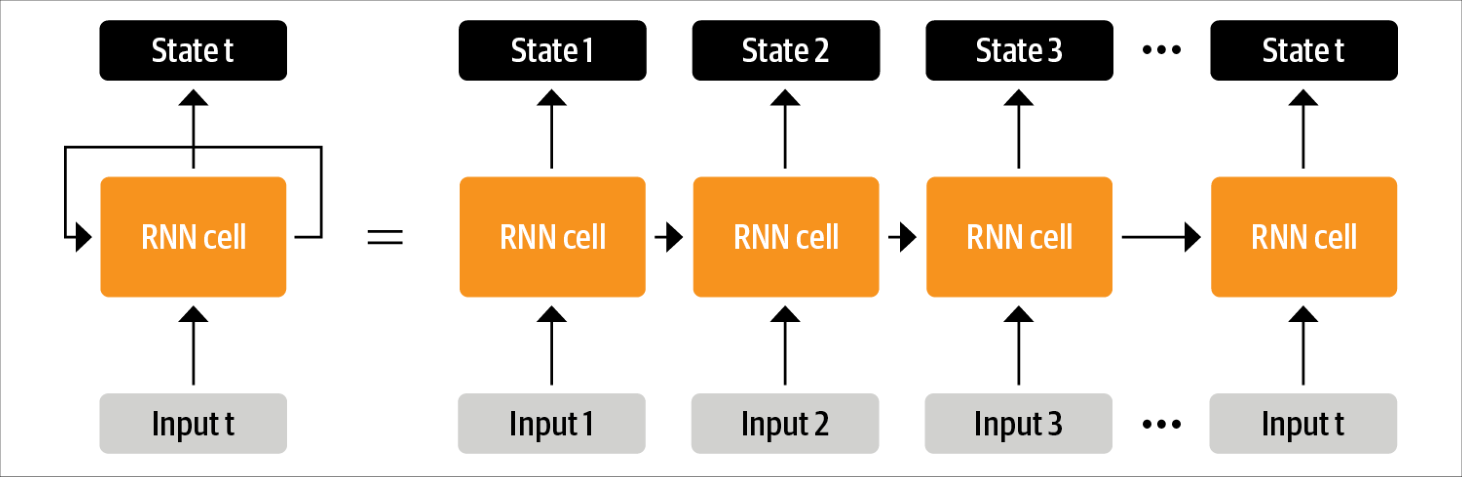
\includegraphics[width=12cm,trim={0.1cm 0.1cm 0.1cm 0.1cm},clip]{./images/unrolling_rnn.png}
\end{center}
\caption{RNN example \cite{tunstallNaturalLanguageProcessing2022}}
\label{fig:rnn_example}
\end{figure}

For tasks such as translation, an encoder-decoder architecture is needed;  the encoder encodes the
input sequence into a numerical representation (called the last hidden state) that gets passed to
the decoder for output sequence generation. Figure~\ref{fig:rnn_encoder_decoder} shows an example of
translating the English statement ``Transformers are great!'' to German. 

\begin{figure}[H]
\begin{center}
  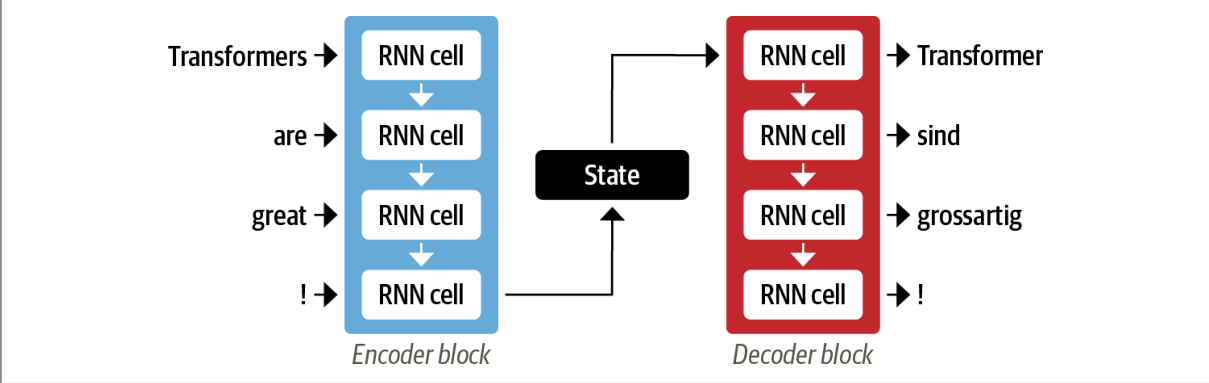
\includegraphics[width=12cm, trim={0.1cm 0.1cm 0.1cm 0.1cm},clip]{./images/encoder-decoder_rnn.png}
\end{center}
\caption{Two RNNs making an encoder-decoder architecture \cite{tunstallNaturalLanguageProcessing2022}}
\label{fig:rnn_encoder_decoder}
\end{figure}

\ac{RNN} has shortcomings when it tries to capture the context of long sequences of information
since the encoder might lose the information at the start while forming the representation.
\ac{RNN}'s weak memory can be addressed by using the attention mechanism that allows the decoder to
access all the hidden states of the encoder. The main goal of attention is to enable the decoder to
prioritize the states using weights it assigns at every decoding timestamp.
Figure~\ref{fig:rnn_encoder_decoder_attention} shows an example for predicting the third token in
the output sequence. Even though attention improves the accuracy of the translations, the
computations are sequential and cannot be parallelized. In addition, most \ac{NLP} tasks require
training models using a large amount of labelled text data that might not be available. Transfer
learning resolves this problem by transferring knowledge acquired from solving one problem to other
related ones.

\begin{figure}[H]
\begin{center}
  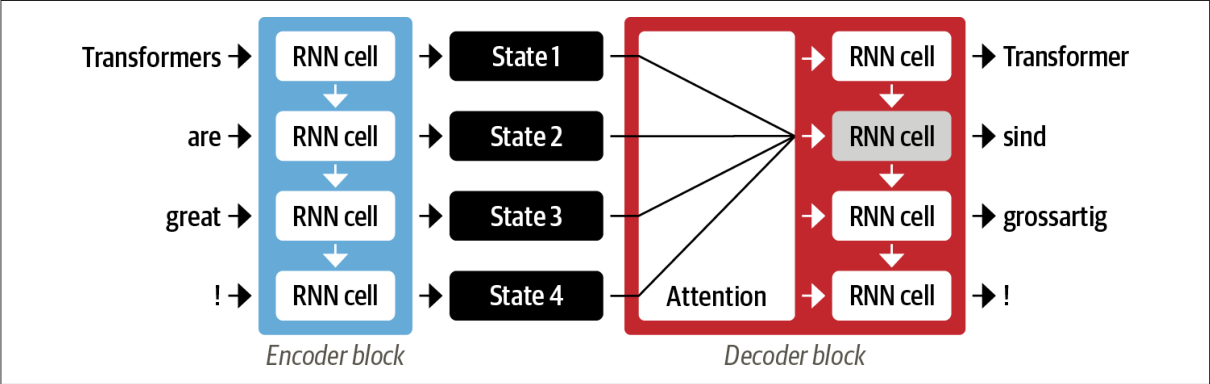
\includegraphics[width=12cm,trim={0.1cm 0.1cm 0.1cm 0.1cm},clip]{./images/encoder-decoder_rnn_attention.png}
\end{center}
\caption{Two RNNs making an encoder-decoder architecture with attention mechanism \cite{tunstallNaturalLanguageProcessing2022}}
\label{fig:rnn_encoder_decoder_attention}
\end{figure}

Transfer learning has been used in computer vision before its introduction to \ac{NLP}. The models
are pre-trained on massive datasets, such as Imagenet
\cite{krizhevskyImageNetClassificationDeep2017} and places database
\cite{zhouLearningDeepFeatures2014} to learn the basic features of images, such as edges and
colours; then, they are fine-tuned on downstream tasks with a smaller dataset.
\citeauth{fengExtractionPluvialFlood2018} use GoogLeNet (Inception-V3 model) \cite{7780677}
pre-trained on ImageNet to train multilayer perceptron, random forest, gradient boosted trees, and
XGBoost with accuracies of 0.8907, 0.9133, 0.9252, and 0.9295, respectively.
\citeauth{ningPrototypingSocialMedia2020} uses VGGNet \cite{simonyanVeryDeepConvolutional2015},
Inception V3, ResNet \cite{heDeepResidualLearning2015}, and DenseNet201
\cite{huangDenselyConnectedConvolutional2018} with 0.91 accuracy.

In 2017 and 2018, several research groups proposed new approaches to use transfer learning for
\ac{NLP}. \ac{ULMFit} \cite{howardUniversalLanguageModel2018} introduced a general framework by
pre-training \ac{LSTM} models for various tasks.
\citeauth{petersenIdentificationExplorationExtreme2021} fine-tune a pre-trained \ac{ULMFit} model
to classify flood-relevant tweets with an accuracy of 0.9499. 

Transformers with transfer learning and their self-attention architecture, proposed by google
researchers \cite{vaswaniAttentionAllYou2017}, made the training process much faster. The idea is to
use attention on all states in the same neural network's layer.
Figure~\ref{fig:encoder_decoder_transformer} shows the self-attention mechanism on both the encoder
and decoder with their outputs fed to feed-forward neural networks.
\citeauth{alamFloodDetectionTwitter2020} fine-tune a pre-trained \ac{BERT}
\cite{devlinBERTPretrainingDeep2019}  model that works on one language with an accuracy of 0.853,
and \citeauth{debruijnGlobalDatabaseHistoric2019b} use a multilingual model with 0.8 F1-score.

\begin{figure}[H]
\begin{center}
  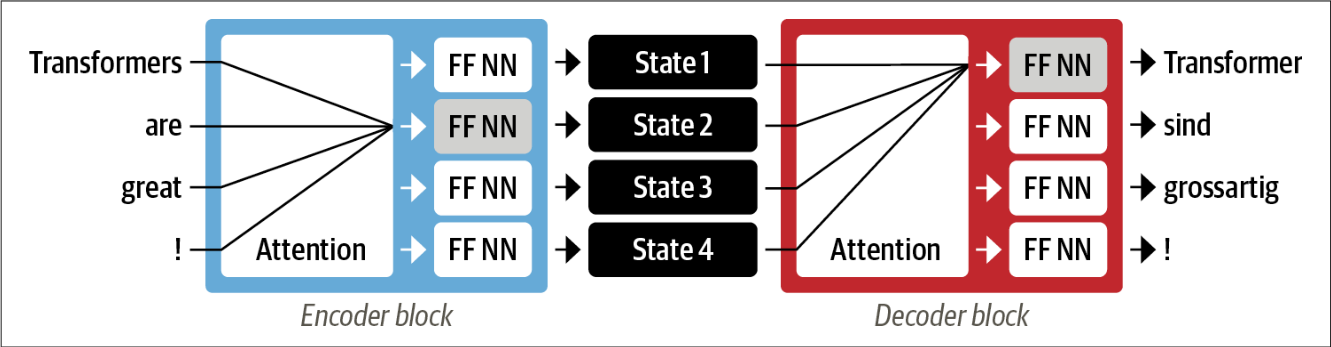
\includegraphics[width=12cm, trim={0.1cm 0.1cm 0.1cm 0.1cm},clip]{./images/encoder-decoder_transformer.png}
\end{center}
\caption{Transformer's encoder-decoder architecture \cite{tunstallNaturalLanguageProcessing2022}}
\label{fig:encoder_decoder_transformer}
\end{figure}


\section{Location Extraction} 
Identifying the locations of disasters is helpful for the disaster
management cycle. Social media enables people to generate \ac{VGI}, which is more advantageous over
the more expensive accuracy testing done by official agencies because contributors have unique local
knowledge.  Detecting a disastrous event and its location as soon as possible can reduce its impact
on society \cite{debruijnGlobalDatabaseHistoric2019b} by informing the citizens and the authority to
prepare for it. During the event, the rescue teams' task becomes easier if they can locate the
endangered people \cite{singhEventClassificationLocation2019}. When the event wanes, assessing the
most impacted spots can enable the authority to make informed decisions on a recovery plan.

Twitter users can assign an accessible property to their tweets, called \texttt{geotag}, a geographical
identification metadata. Adding \texttt{has:geo} to the query sent to the \ac{API} will return geotagged
tweets with metadata about the location, such as its display name, geographical polygon,
latitude, and longitude. The geotag is the most straightforward method to identify the locations 
\cite{fengExtractionPluvialFlood2018}, but unfortunately, only 1\% of the tweets are geotagged
\cite{middletonLocationExtractionSocial2018}.

Locations can be extracted using toponyms, a place's name, in tweets' text by using geoparsing,
which is a process of converting free-text descriptions of places (such as ``twenty miles northeast
of Jalalabad'') into unambiguous geographic identifiers. A toponym can have more than one location
candidate, such as ``Boston'', which is the name of several places, including ``Boston, USA'' and
``Boston, UK''; this fact makes geoparsing tasks on a global scale harder than local ones.
\citeauth{debruijnGlobalDatabaseHistoric2019b} use TAGGS \cite{debruijnTAGGSGroupingTweets2017}, a
geoparsing algorithm, to extract countries, administrative areas, and settlements (i.e. cities,
towns, and villages) mentioned within the tweets' text on a global scale. The process includes
toponym recognition and toponym resolution. Toponym recognition extracts the toponyms that refer to
one or more locations using a gazetteer, a geographical index, or a dictionary. Toponym resolution
predicts the correct location for the toponyms in several steps. A score is assigned to each
possible location using metadata related to the tweet, such as the user's timezone and hometown, the
tweet's coordinates, and mentions of nearby locations. Then, the average score of grouped tweets
mentioning the same toponym within a 24-hour is calculated. Finally, the groups of tweets with the
location that has the highest score are assigned.
\citeauth{petersenIdentificationExplorationExtreme2021} use geotag property, geoparsing using
\ac{NER} on text, and user's profile location to extract toponyms. If the text contains two
toponyms, they pick one randomly if the locations are close with a distance threshold of 1500km.
They use GeoPy\footnote{https://geopy.readthedocs.io/en/stable/} to assign geographical locations to
toponyms, a Python package that is a client for several popular geocoding web services (e.g.,
GoogleV3 and GeoNames). \citeauth{singhEventClassificationLocation2019} use the fact that people
visit the same locations daily to generate a Markov chain model on historical tweets created by the
same user to locate them. 

\section{Text Analysis}

Besides text classification and location extraction, other text analysis techniques extract valuable
information from text data. During hazards, disaster managers can use social media to get insights,
such as how impactful an event is on society. They can visualize the results to understand the
situation and act accordingly. 

\citeauth{grunder-fahrerHowSocialMedia2018} extract multiple relevant pieces of information from
social media and present them to disaster managers via a searchable application. They extract the
following: topics using HDP-CRF algorithm \cite{tehHierarchicalBayesianNonparametric2010}, locations
using Openstreetmap\footnote{https://www.openstreetmap.org/} location markers, time using the social
media metadata, and names of organizations using \ac{NER}. They present the information using
several interactive graphs such as pie charts, word clouds and line graphs.

Dimensionality reduction is a common preprocessing technique to reduce the complexity of textual
data, preparing it for other tasks such as noise reduction, visualization, or clustering.
\citeauth{heusingerDimensionalityReductionContext2022} use random projection to reduce the
dimensions of tweets to predict their hashtags, making them easier to search on Twitter.
\citeauth{omuyaSentimentAnalysisSocial2022} extract features from social media using Principal
Component Analysis to perform sentiment analysis. Sentiment analysis is a popular text analysis
technique that shows people's sentiments during an event. \citeauth{luVisualizingSocialMedia2015}
perform sentiment analysis from Twitter about the Ebola virus using three different sentiment
classifiers to measure the sentiment score of the tweet depending on the majority of the votes.
Also, they calculate the inconsistency between the classifiers using an entropy measure
\cite{argamon-engelsonCommitteeBasedSampleSelection1999}. The positive and negative sentiments are
each presented in a density map using solid blue and red colours, respectively; if the inconsistency
score is above a certain threshold, the colour is blurred.
\citeauth{perinan-pascualAssessingImpactTweets2020} tries to extract the sentiment by calculating
three scores for the tweets: (1) the reliability of how much the tweet discusses a problem during a
hazard, (2) the impact of the tweet by using the user's activity and popularity as well as tweet's
influence \cite{palIdentifyingTopicalAuthorities2011}, (3) and the impact of the
problem using the previous scores. They present the mean of the scores on a time frame basis on a
line graph.

\section{Visualization}
Data is not useful by itself unless meaningful information is extracted from it to accomplish
given tasks. Extracting relevant information for the right time and occasion from heterogeneous
and massive data sources is challenging. Information visualization provides users with an
opportunity to analyse the data by showing different aspects of it. Yet, it doesn't solve the
information explosion by itself; this is where visual analytics comes in by placing the focus on
the relevant information only for the right audience by combining different disciplines, such as
information visualization, data mining, human-computer interaction, and perception and
cognition. It uses multiple disciplines and distributes the work between humans and machines to
improve problem-solving and decision-making \cite{keimVisualAnalyticsDefinition2008}.

Social media has attracted the attention of researchers interested in extracting information using
visualizations and visual analytics. \citeauth{chenSocialMediaVisual2017} contributed a survey
addressing the techniques done on the entities seen in social media (networks, geographic information,
and text) and their applications, such as event detection and situation awareness, which are
relevant from a disaster management point of view. \citeauth{liuBridgingTextVisualization2019}
focus more on providing an overview of text visualization and mining concepts with a web tool to
search for research trends. \citeauth{kucherTextVisualizationTechniques2015} created a web-based
interface containing 440 categorized text visualization techniques by
2019\footnote{https://textvis.lnu.se/}.

\begin{figure}[ht!]
\begin{center}
  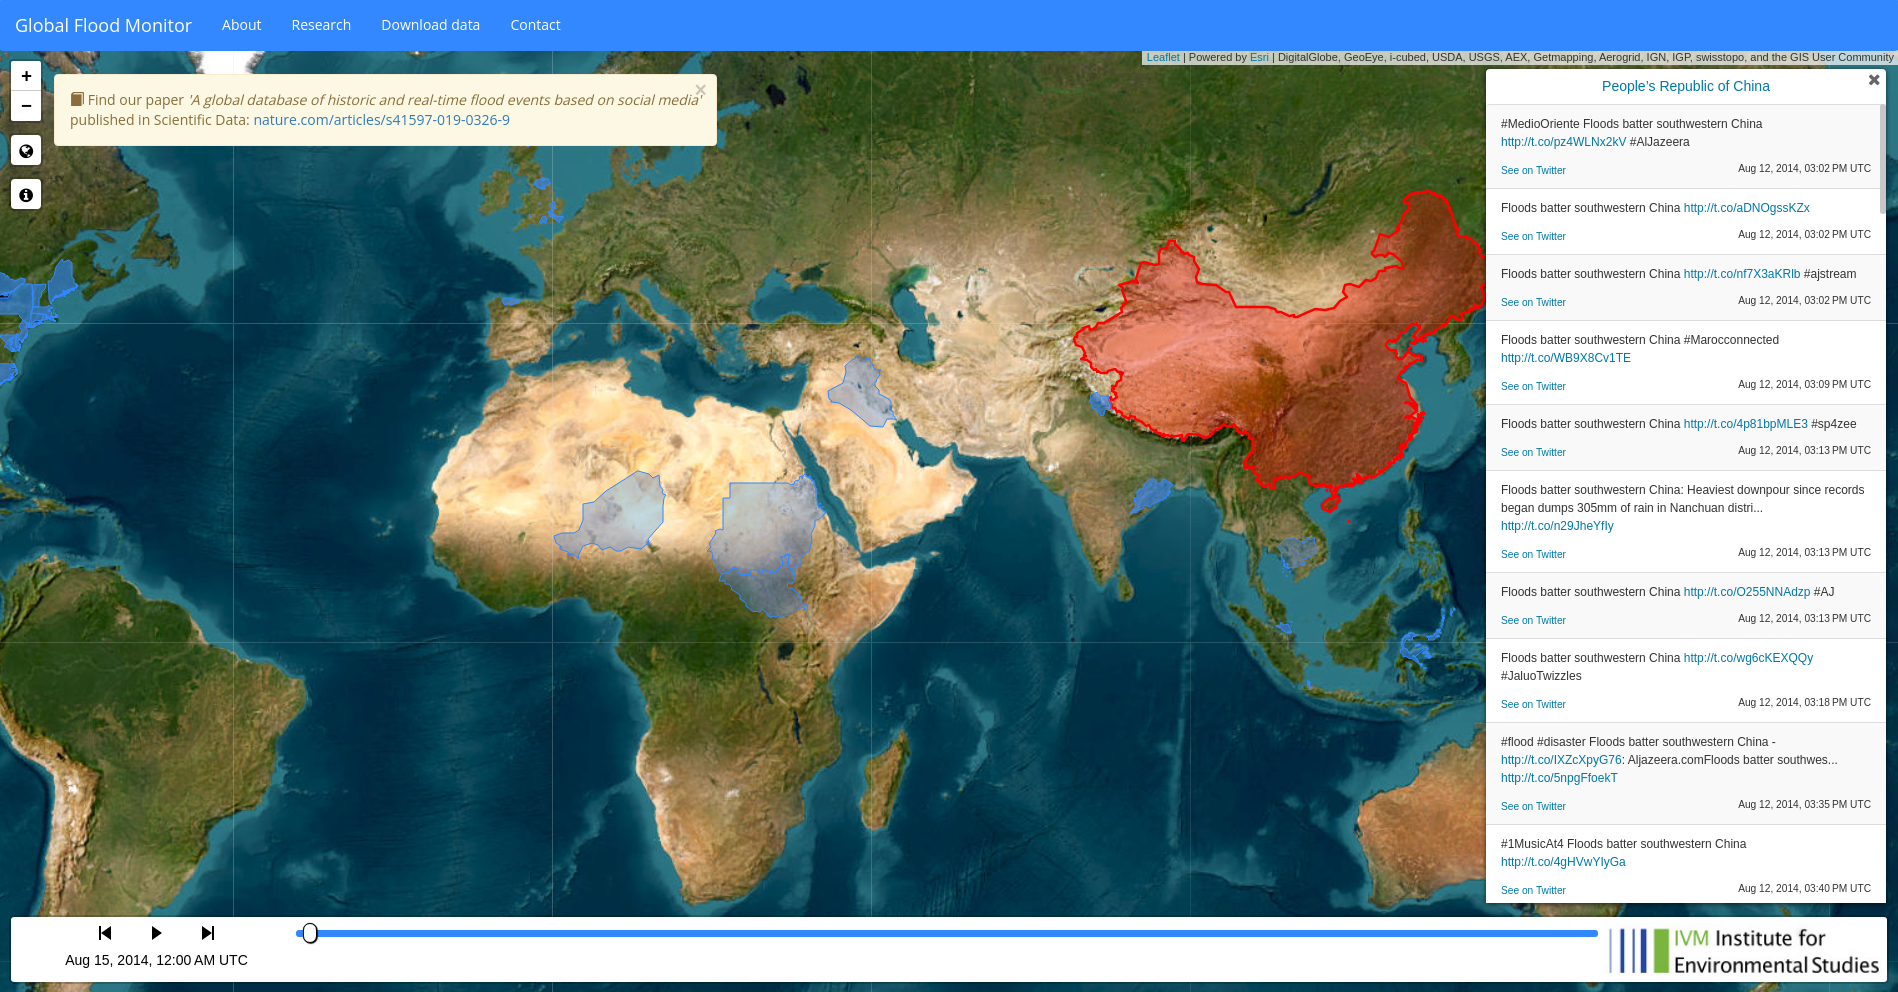
\includegraphics[width=\columnwidth]{images/global.png}
\end{center}
\caption{Global Flood Monitor application showing flood events}
\label{fig:global}
\end{figure}

\citeauth{petersenIdentificationExplorationExtreme2021} provide multiple plots with sophisticated
methods to configure the interface and filter the tweets. Their visualization is powered using the python
libraries, Plotly\footnote{https://plotly.com/python/} and Dash\footnote{https://dash.plotly.com/}.
The app, shown in Figure~\ref{fig:peter}, provides an interface to showcase the different aspects of the
data: spatial via a map, temporal via a histogram, and textual via a list of tweets and word cloud.
They use a scatter map to show the locations extracted from the tweets, where the colour of each
point represents the method used to identify the location. To resolve the problem of tweets
overlapping each other due to the discussion of the same location, the identical points are
spread by adding Gaussian noise to their coordinates points. As for representing the timestamps,
they use a histogram aggregated by each day with a time slider. Researchers can pinpoint repetitive
or interesting topics by navigating the word cloud to see the most frequent keywords or manually
navigating the list of tweets. The plots are interactive, where actions in one of them would
influence others. The data can be filtered in different ways: keywords in the text, the method used
to extract the location, tweet type (a retweet or not), a map, and a histogram. In addition, there is a
drop-down to change the map graph type and the algorithm used to classify the tweets.

\begin{figure}[H]
\begin{center}
  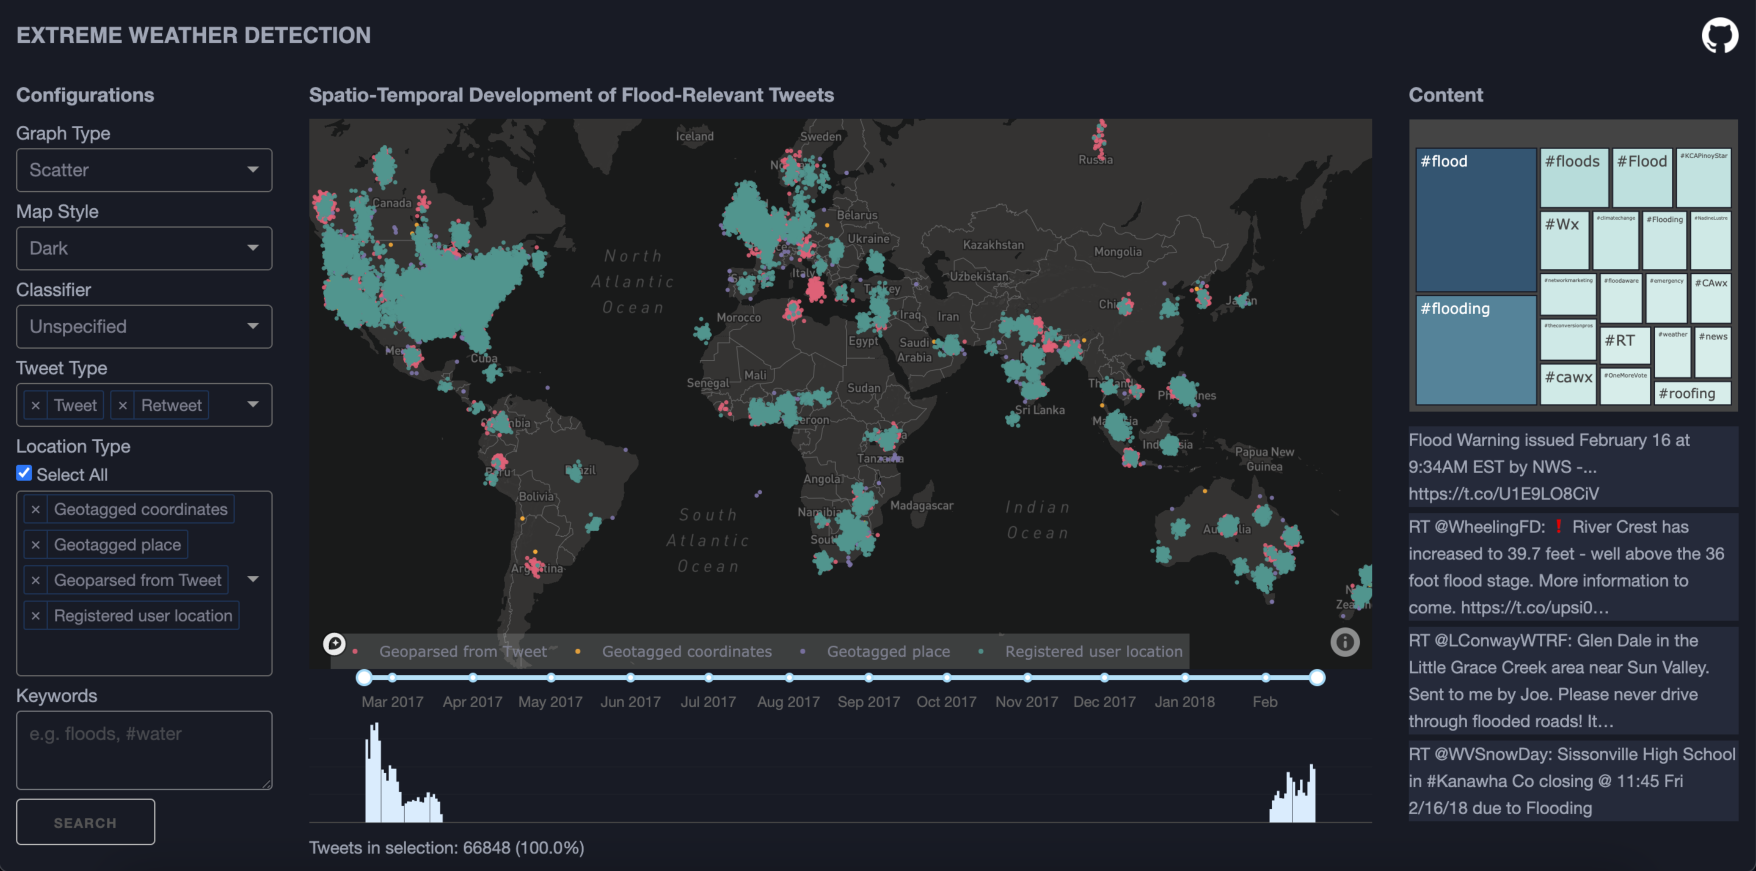
\includegraphics[width=\columnwidth]{./images/peter.png}
\end{center}
\caption{\citeauth{petersenIdentificationExplorationExtreme2021} application}
\label{fig:peter}
\end{figure}

\citeauth{fengExtractionPluvialFlood2018} use leaflet to plot a map showing flooding events as
observed in Figure~\ref{fig:feng}. They use $\text{Getis-Ord Gi}^{\ast}$ \cite{ordLocalSpatialAutocorrelation2010}
to detect statistical hot spots and present them as a choropleth map. The light blue circles
represent the spatio-temporal clusters of events, and the circles with numbers at the centre
indicate clusters of tweets in that area with their total. The markers indicate individual tweets
with a pop-up containing information about it.

\begin{figure}[H]
\begin{center}
  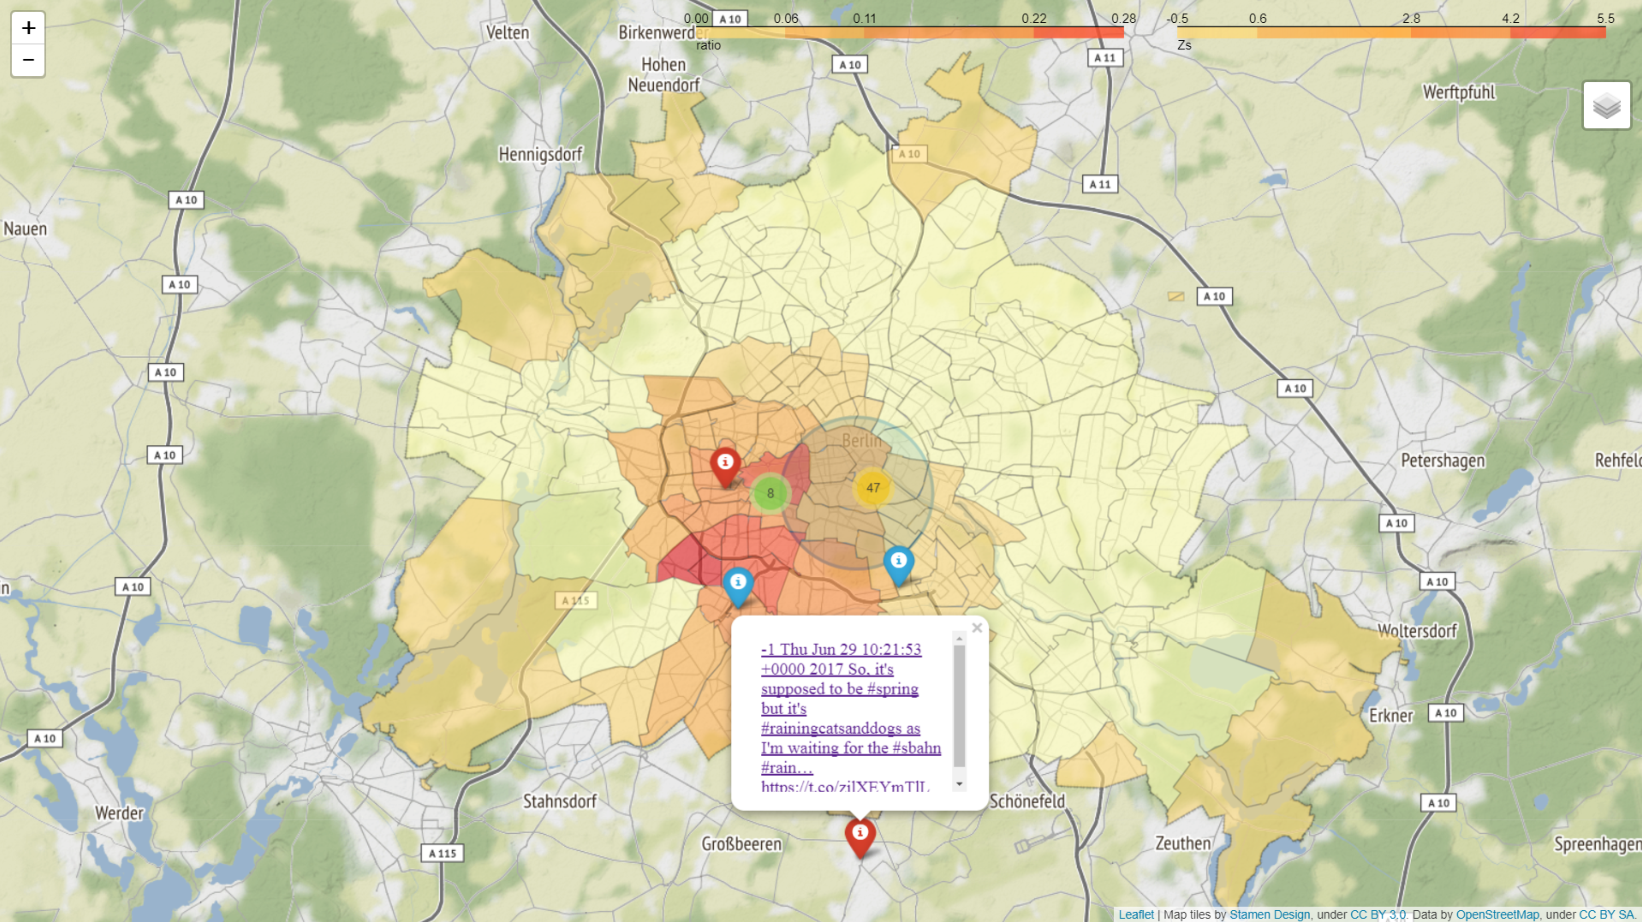
\includegraphics[width=13cm]{./images/feng.png}
\end{center}
\caption{Web map application with pluvial flood in Berlin by \citeauth{fengExtractionPluvialFlood2018}}
\label{fig:feng}
\end{figure}

\citeauth{barkerDevelopmentNationalscaleRealtime2019} visualize the tweets using different map plots
 created by leaflet. The map plot in Figure~\ref{fig:baker_marker} consists of clickable pointers for pop-up boxes of the tweets.

\begin{figure}[H]
\begin{center}
  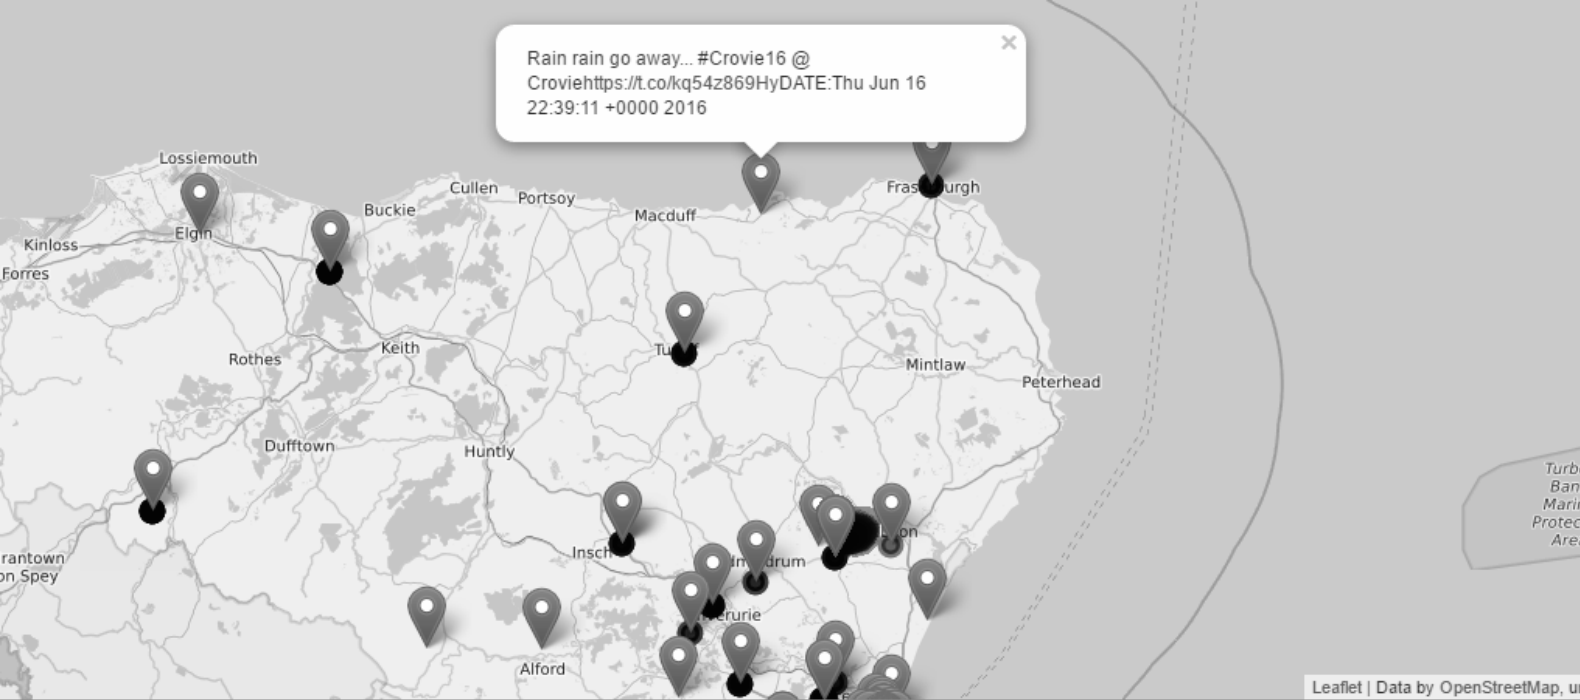
\includegraphics[width=13cm]{images/baker_marker.png}
\end{center}
\caption{Map with tweet markers in by \citeauth{barkerDevelopmentNationalscaleRealtime2019}}
\label{fig:baker_marker}
\end{figure}

The bubble map in Figure~\ref{fig:baker_bubble} displays the tweets with the size of the circles
representing the area of the place and colour indicating the number of tweets talking about the
location.
\begin{figure}[H]
\begin{center}
  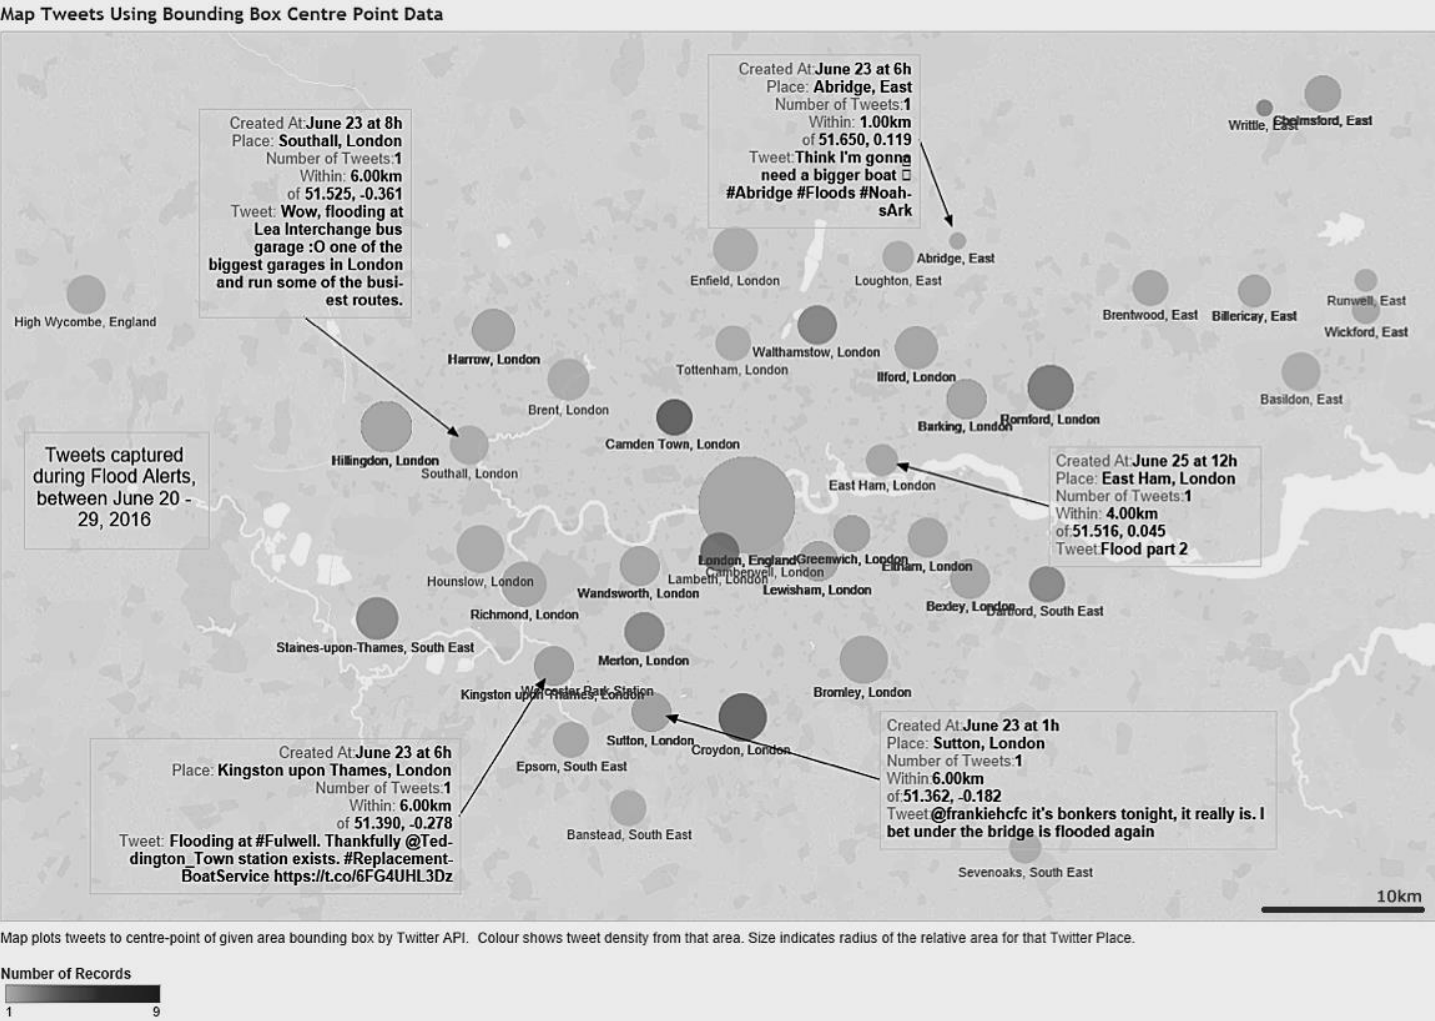
\includegraphics[width=13cm]{./images/baker_bubble.png}
\end{center}
\caption{Bubble map of tweets by \citeauth{barkerDevelopmentNationalscaleRealtime2019}}
\label{fig:baker_bubble}
\end{figure}
